\documentclass{beamer}
\usetheme[hideothersubsections]{AUTheme}
\setbeamertemplate{bibliography item}[text]%,
\setbeamertemplate{footline}[frame number]
\usepackage[scaled]{helvet}
\usepackage{url}
\usepackage{tikz,pgf}
\usepackage{epstopdf}
\usepackage{siunitx}
\usepackage{amsmath}
\usepackage{graphicx,subfigure}
\usepackage[maxcitenames = 1, mincitenames=1,backend=bibtex]{biblatex}
\usepackage{multicol}
\usepackage{wrapfig}
\usepackage{hypcap}
\usepackage{lipsum}
\usepackage[absolute,overlay]{textpos}
\usepackage[justification=centering]{caption}

\captionsetup[figure]{labelformat=empty}

\hyphenation{op-tical net-works semi-conduc-tor}

\usetikzlibrary{arrows}

\AtBeginSection[] {
  \begin{frame}<beamer>
    \frametitle{Section Outline}
    \tableofcontents[currentsection,hideallsubsections]
  \end{frame}
}

\bibliography{../bib/master.bib} % problems here
\newcommand{\citeitem}[1]{[\emph{\Citeauthor*{#1}, \citeyear{#1} }]}

\title[DRTK Driver Assistance]{An On-Line Visual Driver Aid for\\ Safe and Precise Convoy Following in\\ Visibility-Impaired Conditions}
\author[]{Robert Cofield, Scott Martin, David Bevly}
\date{September 18, 2013} 

%%%%%%%%%%%%%%%%%%%%%%%%%%%%%%%%%%%%%%%%%%%%%%%%%%%%%%%%%%%%%%%%%%%%%%%%%%%%%%%%

\begin{document}

%% Title Slide %%
\frame{\titlepage}

%%%%%%%%%%%%%%%%
%% Motivation %%
%%%%%%%%%%%%%%%%

\section{Motivation}

  %% Military 
  \begin{frame}{Motivation}
    \begin{columns}
      \begin{column}{0.5\textwidth}
        \begin{figure}
          \includegraphics[width=\textwidth]{../graphics/convoy_sandstorm_orange.jpg}
          \vspace{-10pt}
          \caption{\tiny Source: \citeitem{convoy_dust_orange}}
        \end{figure}
      \end{column}
      \begin{column}{0.5\textwidth}
        \begin{itemize} \footnotesize
          \item Vehicle convoys, UXO mapping/clearing, strategic vehicle placement, accident avoidance, planting/harvesting
        \end{itemize}
      \end{column}
    \end{columns}
    \begin{itemize} \footnotesize
      \item The ability to precisely follow another vehicle with large separation distances would have an immediate impact on military ground vehicle systems and future automated civilian vehicle systems.
      \item Many current solutions require vehicles to be in sight of one another so perception sensors can obtain range and bearing information
      \item GPS can provide high accuracy relative position information ($<5cm$)
    \end{itemize}
  \end{frame}


%%%%%%%%%%%%%%%%%%%%%%%%%%%%%%%%
%% Literature & Previous Work %%
%%%%%%%%%%%%%%%%%%%%%%%%%%%%%%%%

\section{Literature}

  \subsection{DRTK}

    %% brief explanation
    \begin{frame}{Dynamic Base Real-Time Kinematic GNSS}
      \begin{itemize} \footnotesize
        \item Code based range measurements have meter level accuracy.
        \item Phase based range measurements are near millimeter level accurate, but are ambiguous.
        \item Relative position measurements are formed by differencing range measurements between two receivers.
      \end{itemize}
      \begin{minipage}{0.45\linewidth}
        Integers fixed using LAMBDA search method.
        \begin{itemize} \footnotesize
          \item 2 candidates
          \item Minimum ratio of 3.00
        \end{itemize}
      \end{minipage}
      \begin{minipage}{0.45\linewidth}
        \begin{figure} \centering
        \includegraphics[width=3.5cm]{../graphics/drtk_errors.png}
        \caption{ \footnotesize North Error $\sigma=0.70cm$\\East Error $\sigma=0.68cm$ }
        \end{figure}
      \end{minipage}
    \end{frame}


    \begin{frame}{Fault Detection \& Exclusion}
      \begin{columns}
        \begin{column}{0.5\linewidth}
          \begin{itemize} \footnotesize
            \item Closely coupled architecture allows for monitoring individual satellites
            \item Local errors usually affect individual signals
            \item Exclude solution degrading outliers
            \item Normalized innovation parameter
            \item Scaled by measurement noise
            \item If parameter over threshold, ignore measurement
          \end{itemize}
        \end{column}
        \begin{column}{0.5\linewidth}
          \Large \centering $y_i=\frac{z_i}{\sigma_i}$
          \begin{figure}
            \includegraphics[width=\textwidth]{../graphics/fde_plot.png}
          \end{figure}
        \end{column}
      \end{columns}
    \end{frame}


  \subsection{TDCP}

    %% brief explanation
    \begin{frame}{Time-Differenced Carrier Phase GNSS}
      \begin{figure}[ht] \centering
        \begin{minipage}[b]{0.45\linewidth}
          \includegraphics[width=\textwidth]{../graphics/tdcp_diagram.png}
          \caption{}
        \end{minipage}
        \begin{minipage}[b]{0.5\linewidth}
          \includegraphics[width=\textwidth]{../graphics/tdcp_errors.png}
          \caption{\footnotesize $\Delta$ North Error $\sigma=0.75mm$\\$\Delta$ East Error $\sigma=1.09mm$}
        \end{minipage}
      \end{figure}
      \begin{itemize} \footnotesize
        \item Accurate change in position can be estimated using time differenced carrier phase (TDCP) measurements.
        \item Differencing two measurements across time “removes” atmospheric and SV clock errors, and the integer ambiguity, \textit{assuming the time difference is small.}
      \end{itemize}
    \end{frame}


  \subsection{Virtual Path}

    %% discuss virtual leader & path summation
    \begin{frame}{Construction of Path}
      \begin{figure}
        \includegraphics[width=10cm]{../graphics/path_algorithm.png}
      \end{figure}
      \begin{itemize} \footnotesize
        \item If the change in vehicle position can be obtained with sufficient accuracy, the relative position vector from a previous time can be translated to the current time.
        \item This new RPV is between a past position of the lead vehicle and the current position of the following vehicle, so the effective following distance has been reduced.
      \end{itemize}
    \end{frame}


    \begin{frame}{Errors in Relative Path}
      \begin{itemize}
        \item TDCP errors grow over time, so each measurement epoch incurs more error.
        \item Longer paths and lower speeds accumulate more error.
      \end{itemize}
    \end{frame}


%%%%%%%%%%%%%%%%%%%%%%%%%%%%%%%%%%%%
%% Presentation of final products %%
%%%%%%%%%%%%%%%%%%%%%%%%%%%%%%%%%%%%

\section{GUI}

    % transitional slide from literature
    % Talk about waypoint following with Prowler
    \begin{frame}{Real-Time Implementation}
      \begin{minipage}{0.45\textwidth}
        \centering
        \includegraphics[width=\textwidth]{../graphics/data_algo.png}
      \end{minipage}
      \begin{minipage}{0.45\textwidth}
        \begin{itemize} \small
          \item DRTK, TDCP errors analyzed by splitting single antenna between 2 receivers
          \item Unmanned Following
          \item Waypoint-based control
          \item No intuitive method for quickly tuning algorithms \& visualizing errors
        \end{itemize}
      \end{minipage}
    \end{frame}


  \subsection{Design}

    %% ConOps
    \begin{frame}{Concept of Operation}
      \begin{figure}
        \includegraphics[width=0.8\textwidth]{../graphics/blackbox_flowchart.png}
      \end{figure}
      \begin{columns}  
        \begin{column}{0.5\textwidth}
          \footnotesize User inputs
          \begin{itemize} \footnotesize
            \item Critical alert values\\ ($\mu_{crit}~,~d_{crit}$)
            \item Warning alert values\\ ($\mu_{warn}$~,~$d_{warn}$)
          \end{itemize}
        \end{column}
        \begin{column}{0.5\textwidth}
          \footnotesize Relay to user
          \begin{itemize} \footnotesize
            \item Lateral path deviation alerts
            \item Path separation distance alerts
          \end{itemize}
        \end{column}
      \end{columns}
    \end{frame}

    % what led to simple GUI
    % mention SBIR?
    \begin{frame}{Initial Design Goals}
      \begin{columns}
        \begin{column}{0.5\linewidth}
          Army SBIR A131-027-133
          \begin{itemize} \footnotesize
            \item Yuma, AZ desert --- extremely dusty, zero visibility.
            \item Convoy driving with 10-200m desired longitudinal spacing.
            \item Needed quickly intelligible display of distance to adjacent lead vehicle.
          \end{itemize}
          Key Goals
          \begin{itemize} \footnotesize
            \item Relay distance, deviation alerts
            \item Intuitive, easy to understand display \& controls
            \item Graphical representation of path
          \end{itemize}
        \end{column}
        \begin{column}{0.5\linewidth}
          \begin{figure}
            \includegraphics[width=\textwidth]{../graphics/initial_concept.png}
            \caption{\footnotesize Initial concept for simple GUI}
          \end{figure}
        \end{column}
      \end{columns}
    \end{frame}

    \begin{frame}{Design Procedure}

      Primary Refinement Loop
      \begin{enumerate} \footnotesize
        \item Design modification and/or feature addition
        \item Implement modifications
        \item Validate display information
        \item Perform human testing
        \item Post processing analysis
        \item Qualitative feedback
      \end{enumerate}        

      Rejected Features
      \begin{itemize}
        \item Velocity scaling
        \item Leader always visible
        \item Most feature additions can be turned off
      \end{itemize}
      
      % Position solution & path debugging features

    \end{frame}

  %%% Qt GUI %%%%
  \subsection{Qt}

    \begin{frame}{Qt-Based GUI --- Data Display}
      \begin{figure}[ht] \centering
        \includegraphics[width=4in] {../graphics/final_design_data.png}
        \caption{Qt GUI in normal operation} \label{fig:qt_data_display}
      \end{figure}
    \end{frame}

    \begin{frame}{Qt-Based GUI --- Controls}
      \begin{figure}[ht] \centering
        \includegraphics[width=4in] {../graphics/final_design_opts.png}
        \caption{Qt GUI displaying view control data} \label{fig:qt_controls}
      \end{figure}
    \end{frame}


  %%% Google Earth GUI %%%
  \subsection{Earth}

    \begin{frame}{Google Earth GUI --- Display}
      \begin{figure}
        \includegraphics[width=7.5cm]{../graphics/earth_display.png}
      \end{figure}
    \end{frame}

    \begin{frame}{Google Earth GUI --- Control}
      \begin{figure}[!htb] %% This is the best way to do this.
        \minipage{0.32\textwidth} \centering
          \includegraphics[height=0.85\textheight]{../graphics/earth_data.png}
          \caption{\tiny Data display tab}
        \endminipage\hfill
        \minipage{0.32\textwidth} \centering
          \includegraphics[height=0.85\textheight]{../graphics/earth_parameters.png}
          \caption{\tiny Parameter input tab}
        \endminipage\hfill
        \minipage{0.32\textwidth} \centering
          \includegraphics[height=0.85\textheight]{../graphics/earth_view.png}
          \caption{\tiny View control tab}
        \endminipage
      \end{figure}
    \end{frame}

    %% introduce interpolation
    \begin{frame}{Interpolation}
      % \begin{columns}
        % \begin{column}{0.5\linewidth}
          \begin{itemize} \footnotesize
            \item Introduction of satellite imagery made user highly aware of update rate.
            \item Interpolation used to smooth courses, positions, and path.
            \item Introduce lag of one timestep.
          \end{itemize}
          \vspace{-20pt}
          \begin{figure}[ht] \centering
            \includegraphics[width=6cm] {../graphics/middleware_diagram.png}
            \caption{\footnotesize Interpolation Algorithm}
          \end{figure}
        % \end{column}
        % \begin{column}{0.5\linewidth}

        % \end{column}
      % \end{columns}
    \end{frame}


%%%%%%%%%%%%%%%%%%%%%%%%%%%%%%%%%%%
%% Tests that were run & Results %%
%%%%%%%%%%%%%%%%%%%%%%%%%%%%%%%%%%%

\section{Experimentation}


  \begin{frame}{Experimentation}
    \begin{figure}[ht] \centering
      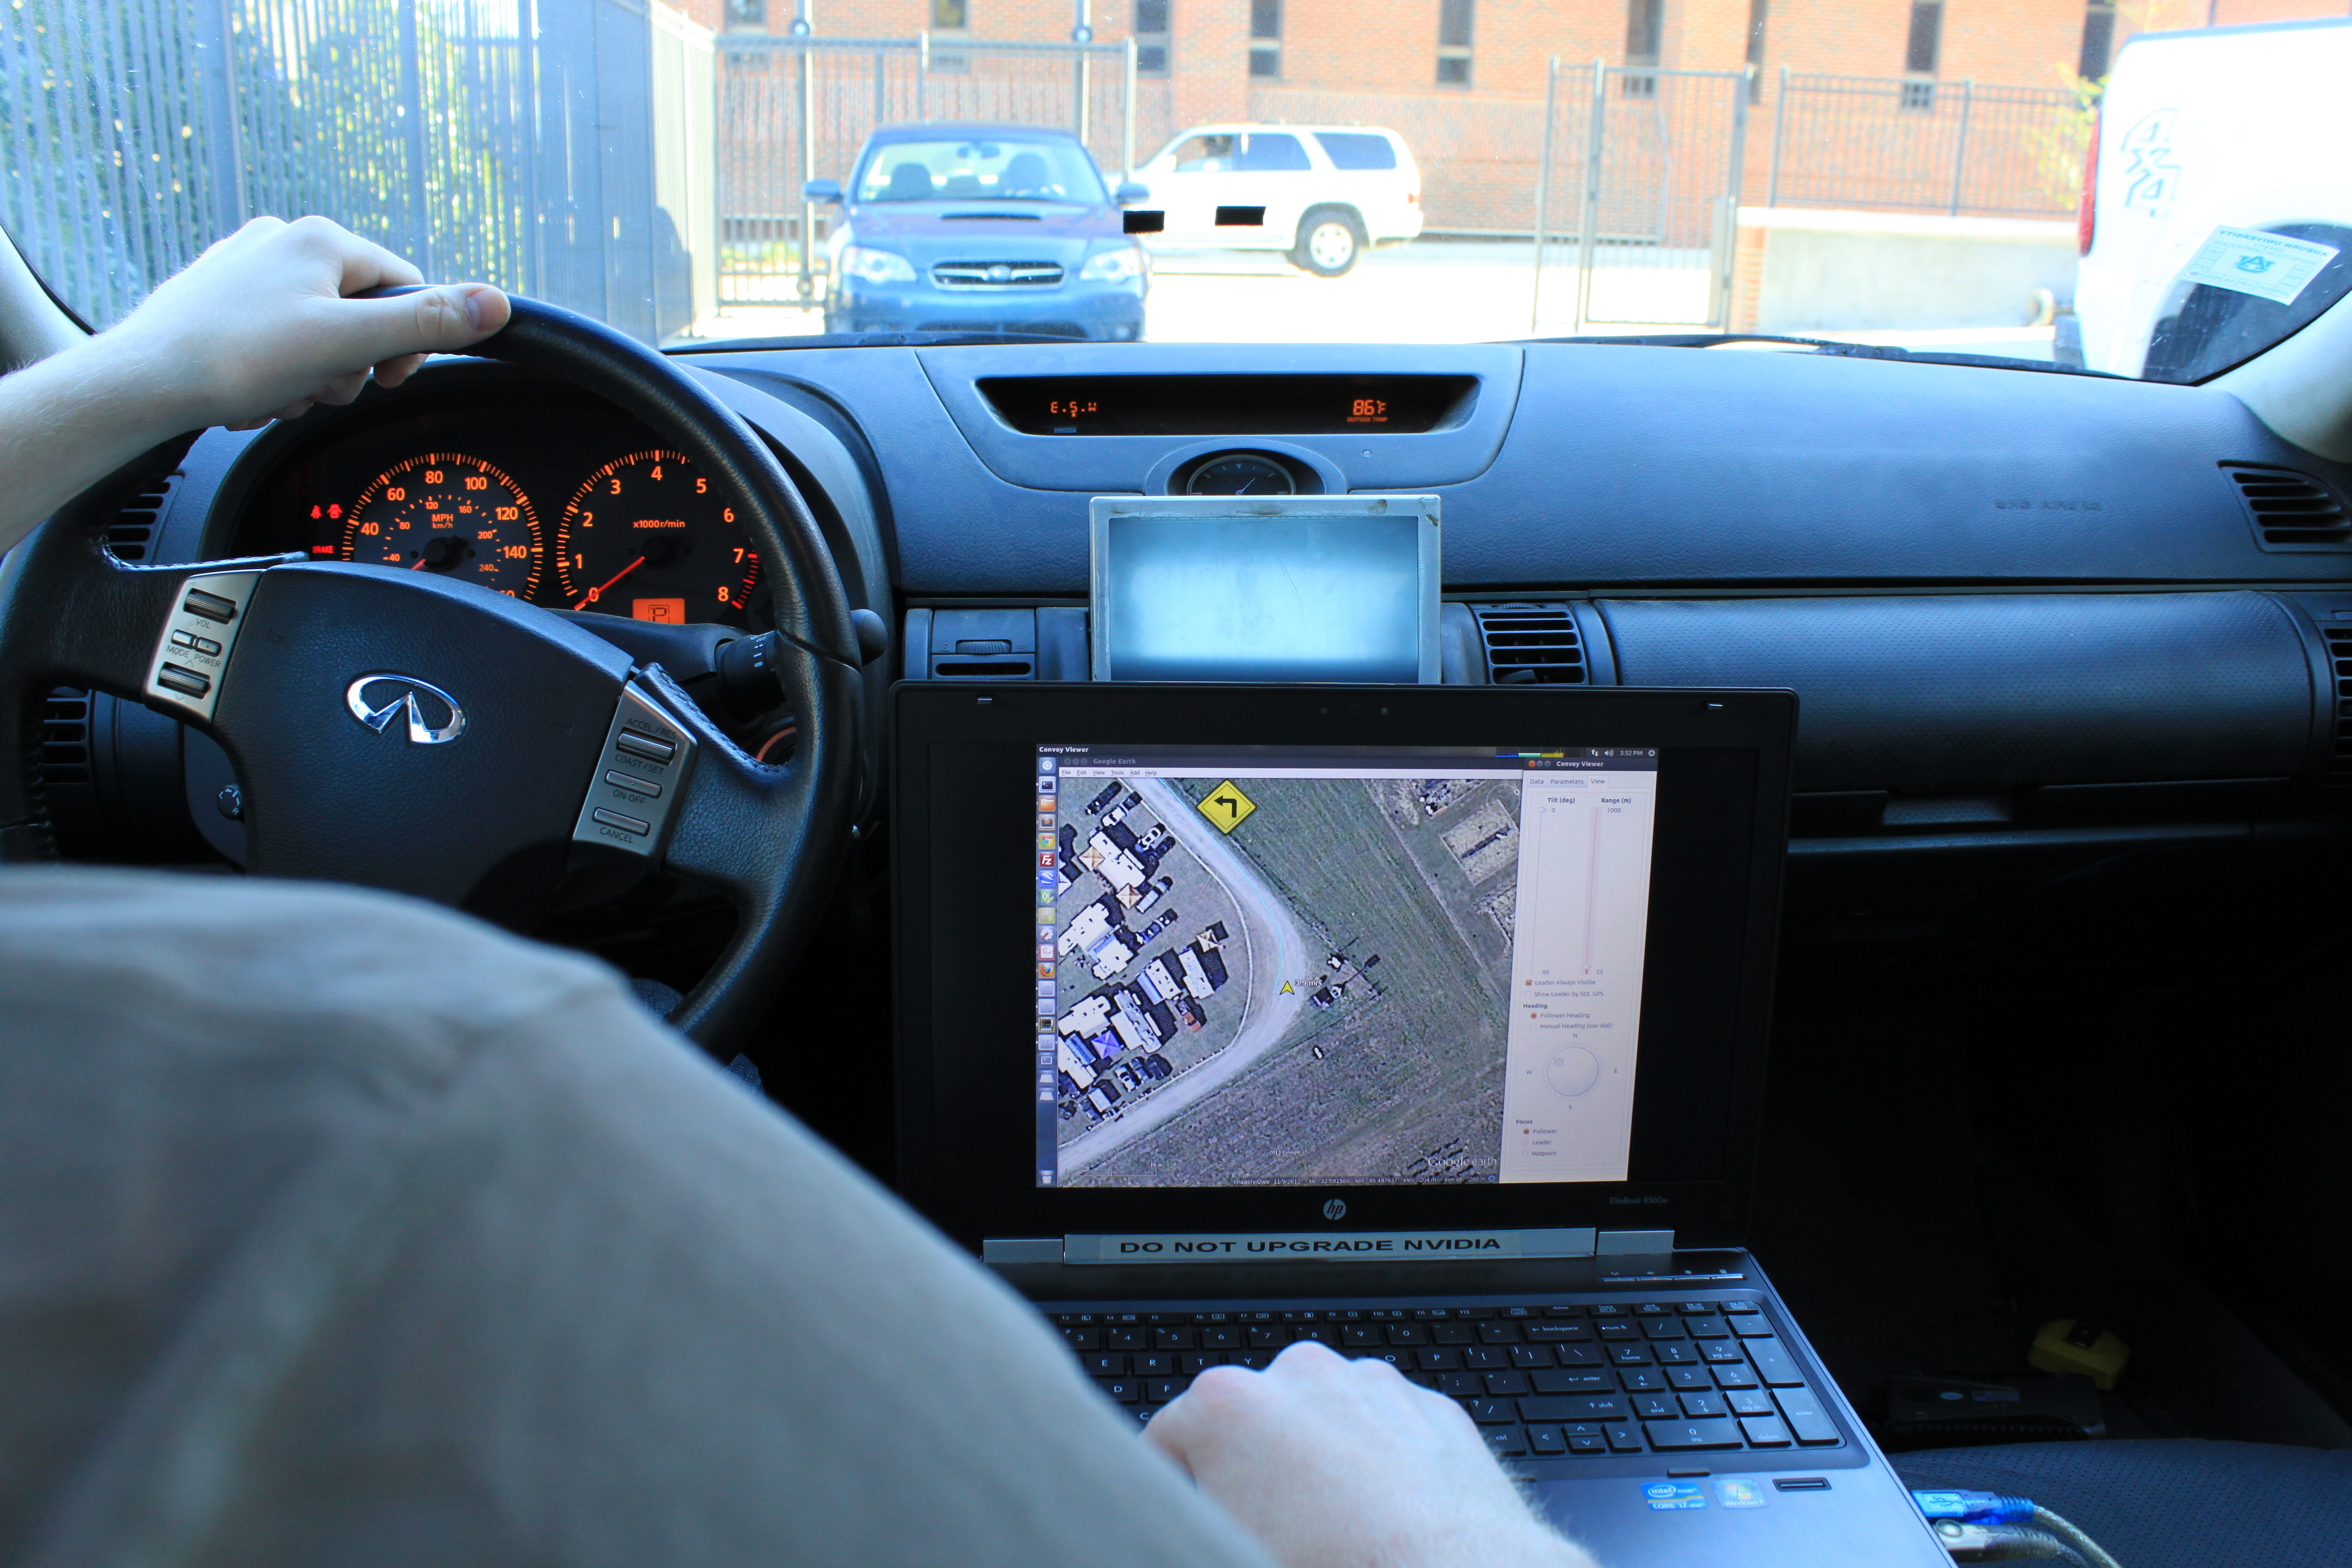
\includegraphics[width=5cm] {../graphics/driver_view.jpg}
      \caption{\scriptsize View from the driver's seat}
    \end{figure}
    \vspace{-20pt}
    \begin{itemize} \footnotesize
      \item 3 vehicle platforms used: Infiniti G35 (sedan), Hyndai Sonata (SUV), Chevrolet Corvette (coupe)
      \item 11 individual test drivers
      \item Road friction coefficient values set to $\mu_{warn}=0.5,\mu_{crit}=1.0$
      \item 3 testing procedures, performed with each GUI (and without aid where applicable)
    \end{itemize}
  \end{frame}

  \begin{frame}{Hardware \& Setup}
      \begin{minipage}{0.45\textwidth}
        \centering
        \includegraphics[width=4cm]{../graphics/hardware_flow.png}
      \end{minipage}
      \begin{minipage}{0.45\textwidth}
        \begin{itemize}
          \item Novatel Propak v3 (OEMV board) L1/L2
          \item Pinwheel Antenna
          \item Digi Extend 900 Mhz radio
        \end{itemize}
      \end{minipage}
      \begin{figure}
        \includegraphics[width=4cm]{../graphics/lead_hardware.jpg}
      \end{figure}
  \end{frame}


  %%% Lane Change Test %%%
  \subsection{Lane Change Test}

    \begin{frame}{Lane Change Test --- Procedures}
      \vspace{-30pt}
      \begin{figure}
        \input{../graphics/lane_change_diagram}
      \end{figure}
      \vspace{-40pt}
      \begin{itemize} \small
        \item Lane change maneuver is visually obscured from follower.
        \item Following driver signalled to begin once maneuver completed.
        \item 6 cones spaced at $\approx10m$.
        \item Results treated as pass/fail.
      \end{itemize}
      % text describing test
    \end{frame}
    
    % What the drivers saw in each GUI during the lane change
    \begin{frame}{Lange Change Test --- Driver View}
      \begin{figure}[ht] \centering
        \begin{minipage}[b]{0.45\linewidth} \centering 
          \includegraphics[width=\textwidth]{../graphics/lane_change.png}
          \caption{Google Earth GUI approaching the lane change maneuver}
        \end{minipage}
        \hspace{0.5cm}
        \begin{minipage}[b]{0.45\linewidth} \centering
          \includegraphics[width=\textwidth]{../graphics/lane_change_mono.png} 
          \caption{Qt GUI approaching the lane change maneuver}
        \end{minipage}
      \end{figure}
    \end{frame}

    % present data
    \begin{frame}{Lane Change Test --- Results}
      \begin{itemize} \footnotesize
        \item Ran test with 4 drivers.
        \item Cone placement and start/end points remained constant.
        \item Runs eliminated in which driver ... 
      \end{itemize}
      \vspace{-10pt}
      \begin{table}[htbp] \centering \footnotesize
        % \caption{Cone pairs chosen in the lane change replication test}
        \begin{tabular}{rc|cc}
          GUI&    Run \#  &     Leader&    Follower \\\hline\hline
          Earth&      1       &       1   &    3 \\
               &      2       &       3   &    4 \\ \hline
          Qt   &      3       &       2   &    3 \\
               &      4       &       5   &    5 \\ \hline   
        \end{tabular}
        \label{tab:lanechangeresults}
      \end{table}
      \begin{itemize} \footnotesize
        \item Drivers reported path appeared to be erroneous relative to satellite imagery (e.g., off the road).
        \item Google Earth positioning errors found to vary up to $50m$ \citeitem{ge_accuracy}.
        \item Typically low speeds when deciding where to turn $(<10m/s)$.
      \end{itemize}
    \end{frame}


  %%% Precision Following Test %%%

  \subsection{Precision Foll. Test}

    \begin{frame}{Precision Following Test --- Procedures}
      \begin{figure}
        \includegraphics[width=10cm]{../graphics/precision_following_diagram.png}
      \end{figure}   
      \begin{itemize} \footnotesize
        \item Two-lane track similar to US interstate.
        \item Performed with each GUI individually, and without aid as control.
        \item Run with fewest combined alerts selected as `best' for each.
      \end{itemize}
    \end{frame}

    % present data
    \begin{frame}{Precision Following Test --- Results}
      \begin{columns}
        \begin{column}{0.5\textwidth}
          \begin{figure}
            \includegraphics[width=\textwidth]{../graphics/precision_following_alert_percents.png}
          \end{figure}
            % discuss results from both
          \begin{itemize} \footnotesize
            \item Kernel smoothed PDF estimates.
          \end{itemize}
        \end{column}
        \begin{column}{0.5\textwidth}
          \begin{figure}
            \includegraphics[width=\textwidth]{../graphics/precision_following_mu_distribution.png}
            % \caption{$\mu$ PDF's for best runs}
          \end{figure}
          \vspace{-20pt}
          \begin{figure}
            \includegraphics[width=\textwidth]{../graphics/precision_following_dev_pdf.png}
          \end{figure}
        \end{column}
      \end{columns}
    \end{frame}


  %%% Zero Landmark Test %%%

  \subsection{Zero Landmark Test}
    \begin{frame}{Zero Landmark Test --- Procedures}
      % \vspace{-20pt}
      \begin{itemize}
        \item No lane markings.
        \item Wide, open expanse of asphalt.
        \item Conducted at night --- minimized visual cues.
        \item Highly erratic speed, course.
      \end{itemize}
      \begin{figure}
        \centering
        \includegraphics[width=0.55\textwidth]{../graphics/zero_landmark_path.png}
      \end{figure}     
    \end{frame}

    % present data
    \begin{frame}{Zero Landmark Test --- Results}
      \begin{columns}
        \begin{column}{0.5\textwidth}
          \begin{figure}
            \includegraphics[width=\textwidth]{../graphics/zero_landmark_alert_percents.png}
          \end{figure}
            % discuss results from both
          \begin{itemize} \scriptsize
            \item Kernel smoothed PDF estimates.
          \end{itemize}
        \end{column}
        \begin{column}{0.5\textwidth}
          \begin{figure}
            \includegraphics[width=\textwidth]{../graphics/zero_landmark_mu_distribution.png}
            % \caption{$\mu$ PDF's for best runs}
          \end{figure}
          \vspace{-20pt}
          \begin{figure}
            \includegraphics[width=\textwidth]{../graphics/pdf_zero_landmark_deviation.png}
          \end{figure}
        \end{column}
      \end{columns}
    \end{frame}



%%%%%%%%%%%%%%%%
%% Conclusion %%
%$%%%%%%%%%%%%%%
\section{Conclusion}

  \begin{frame}{Future Work}
    \begin{itemize}
      \item Reduce latency in combined system.
      \item Increase receiver frequency used.
      \item Combine simplicity of Qt GUI with aesthetics and orientability of Earth GUI.
    \end{itemize}
  \end{frame}

  \begin{frame}{}
    \centering \Huge Questions?
  \end{frame}

\end{document}




%%%%%%%%%%%%%%%%%%%%%%%%%%%%%%%%%%%%%%%%%%%%%%%%%%%%%%%%%%%%%%%%%%%%%%%%%%%%%%%%

%% Font Sizes
% \tiny
% \scriptsize
% \footnotesize
% \small
% \normalsize
% \large
% \Large
% \LARGE
% \huge
% \Huge